\section{Numerical Approximations: Euler's Method}
    Sometimes analytical solutions are not possible so we can use numerical approximations to get close to the actual solution. One of these approximations is called \textbf{Euler's Method}. The basis of Euler's Method is using the differential equation to create a tangent line at the initial value $(t_0, y_0)$, and use it to create an approximation for another point $(t, y)$.
    \begin{equation*}
        y = y_0 + f(t_0, y_0)(t - t_0)
    \end{equation*}
    where $\frac{dy}{dt} = f(t_0, y_0)$. For a better approximation we can repeat this $n$ times instead of just doing it once. So, if we needed to find the solution at $t$, we could use Euler's Method with $n$ steps by
    \begin{equation*}
        y_{i+1} = y_i + f(t_i, y_i)(t_{i+1} - t_i)
    \end{equation*}
    now if we use equal intervals
    \begin{equation*}
        y_{i+1} = y_i + f(t_i, y_i)h
    \end{equation*}
    where $h$ is $(t - t_0) / n$. Or,
    \begin{equation*}
        y = y_0 + \sum_{i=1}^n f(t_i, y_i)h
    \end{equation*}
    \begin{center}
        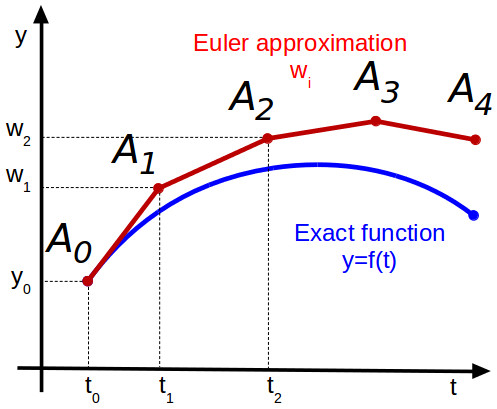
\includegraphics[width=200pt]{euler.jpg}
    \end{center}
    As you increase $n$, the approximation gets better. The Euler method uses the solution that passes through step to approximate the solution that we are looking for. For converging solutions, this works well since all the solutions converge to similar values, while this causes large errors for diverging situations since each step takes you further from the solution.